\section{算法实现}\label{sec:algo-impl}

\subsection{多轨迹收集}

\begin{figure}[h]
\centering
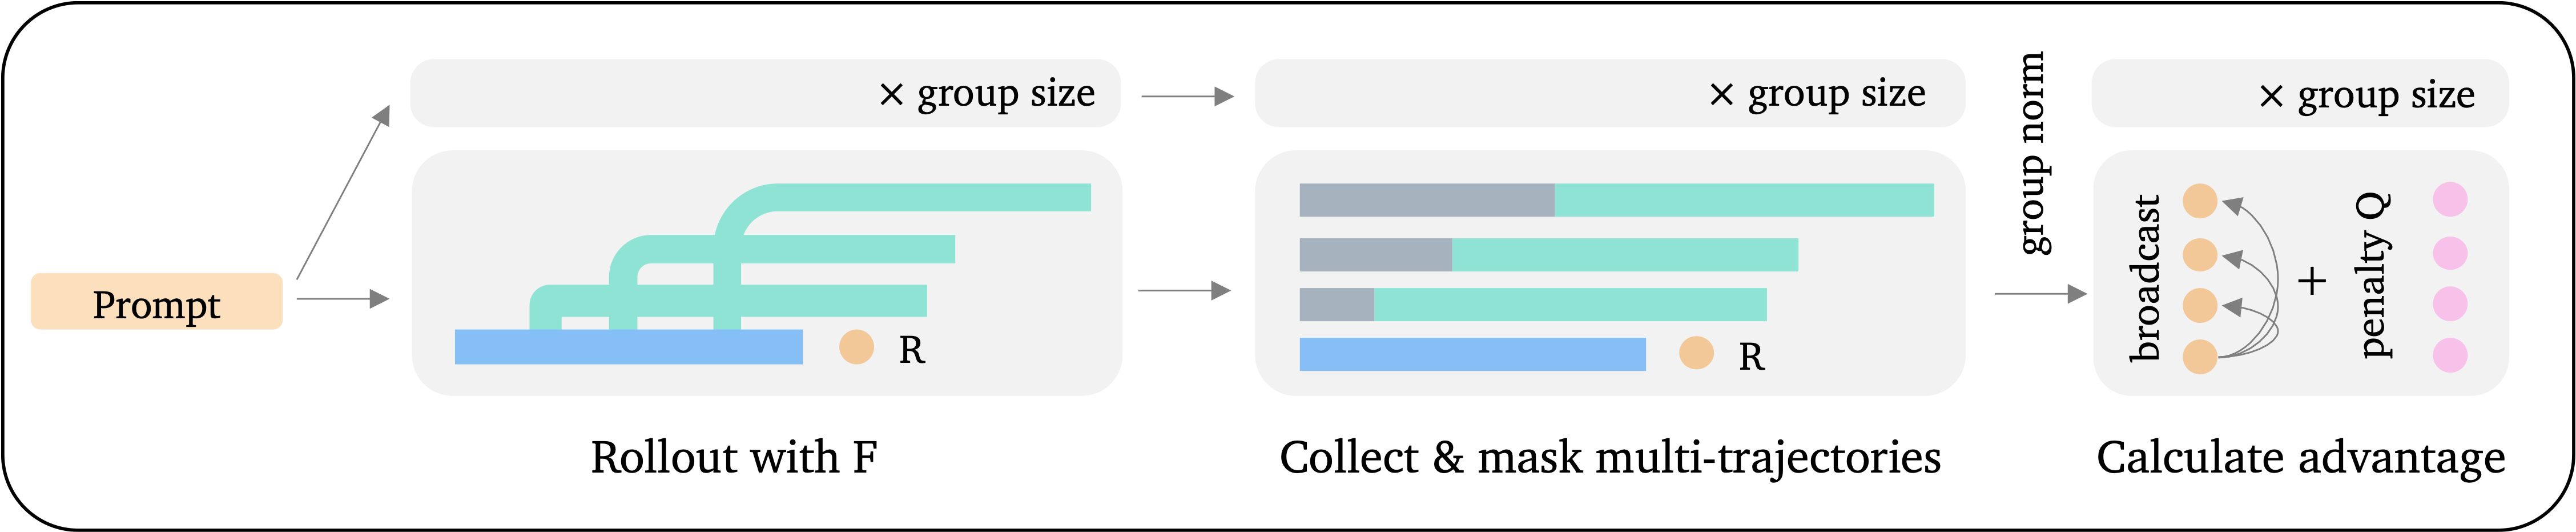
\includegraphics[width=1\columnwidth]{figs/multitraj.png}
\end{figure}

在模型训练的实际实现中，我们不将所有子轨迹拼接为一个序列，而是如上所示，将它们保留为独立的、因果条件化的序列。因此，带有上下文折叠的训练不能直接兼容现有训练基础设施（例如 VeRL）。

\subsection{异步长程智能体 rollout}\label{sec:async-rollout}

\begin{figure}[h]
\centering
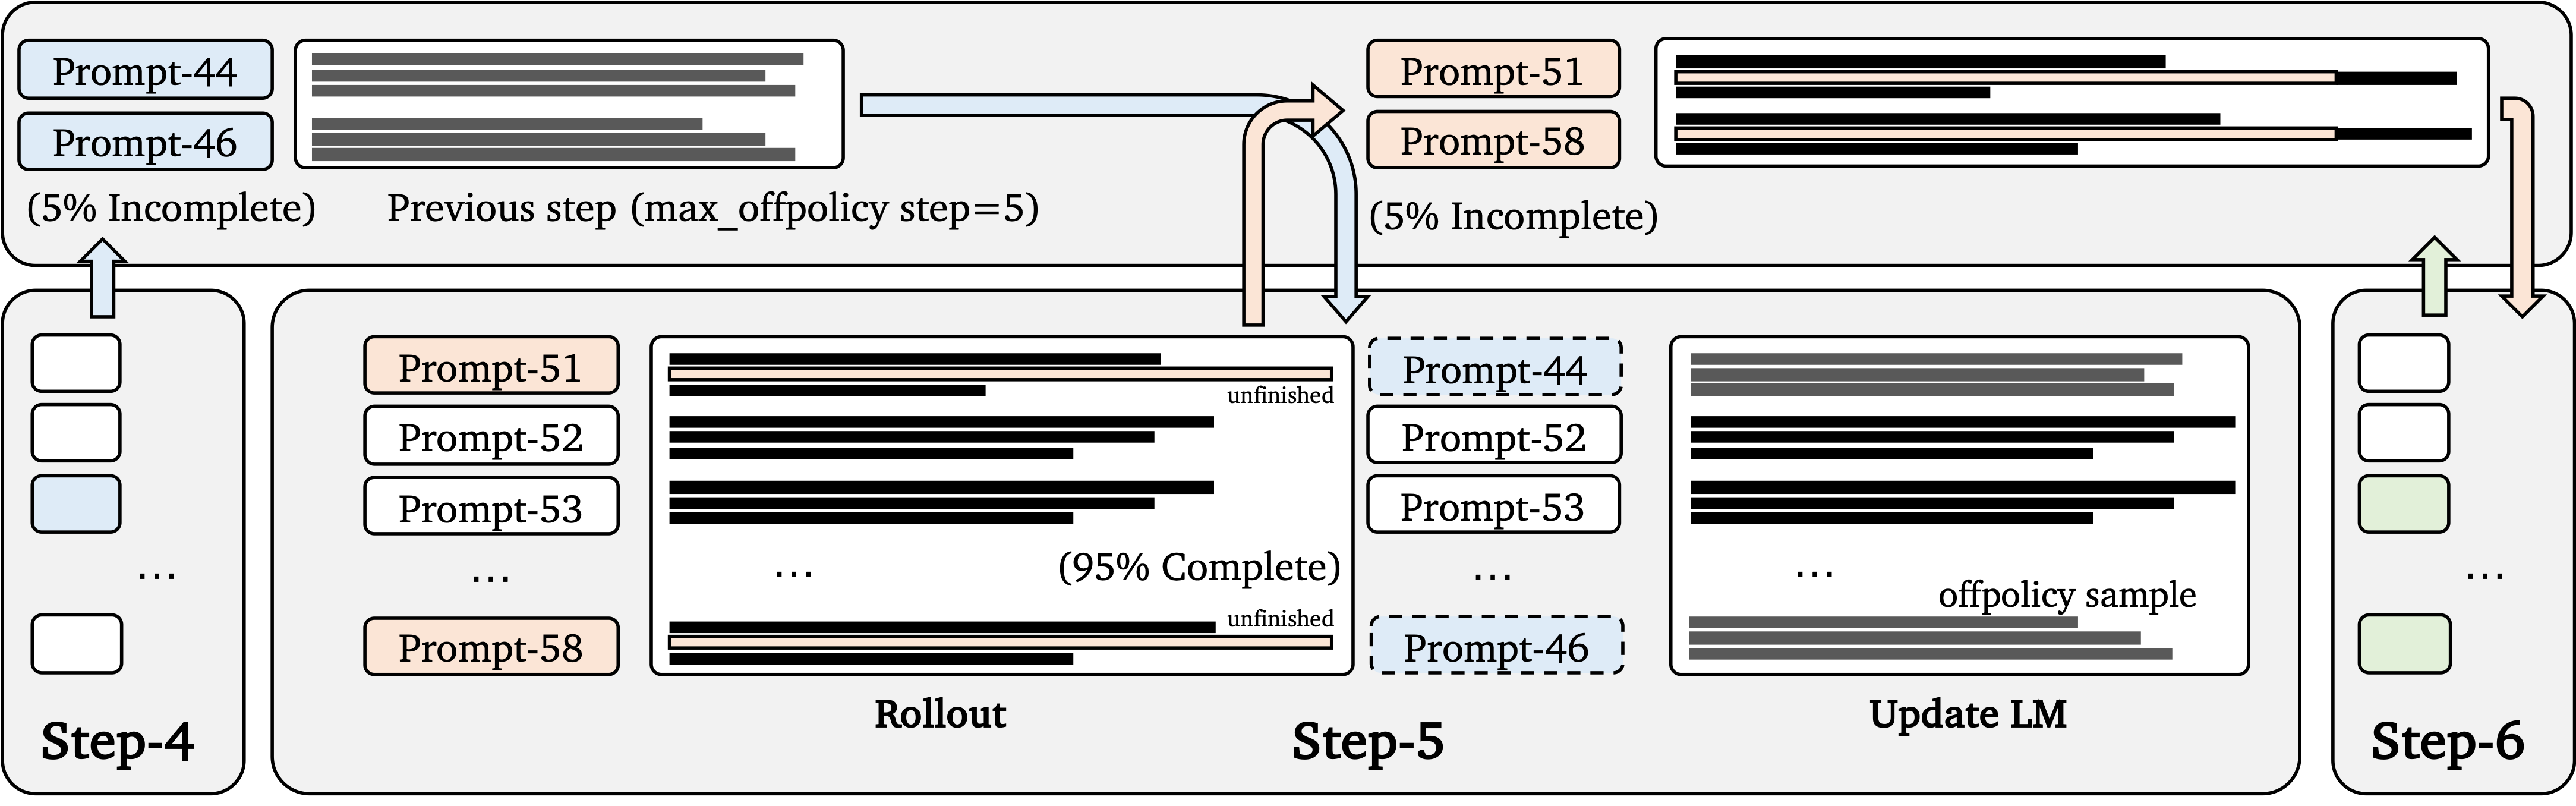
\includegraphics[width=1\columnwidth]{figs/async.png}
\end{figure}

长程智能体的 rollout 时间并不均衡，这会在计算中产生“气泡”：较快作业要等待最慢作业结束。在训练设置中，我们通过增加一个额外的独立 rollout 进程缓解这一问题：主 rollout 进程在完成 95\% 的提示后停止（该超参数会根据 GPU 配置调整），剩余作业由独立进程处理。用于更新 LM 的数据同时包括：（i）当前 batch 的 95\%；（ii）由独立 rollout 在上一步完成的提示。注意后者是 off-policy 的；我们将最大 off-policy 步数设为 5，观察到相较完全 on-policy 数据训练没有性能下降。

\section{提示工程}
\label{sec:pe}

\subsection{BrowseComp-Plus 工作流}
BrowseComp-Plus 的提示受 Claude Deep-Research 启发并在其基础上修改。使用 Seed-OSS-36B 时，我们的系统提示达到 0.478 准确率，而 BrowseComp-Plus 的默认系统提示仅约 0.08。

{\footnotesize
\begin{Verbatim}[breaklines, breakanywhere]
阶段 1：拆解与策略

1.  拆解查询：
    * 分析用户提示，识别核心问题。
    * 分离关键实体、概念及其相互关系。
    * 明确列出所有约束、条件和所需数据点（如日期、数量、特定名称）。
2.  提出假设与头脑风暴：
    * 基于已有知识，构想可能带来相关信息的搜索方向、关键词、同义词和相关主题。
    * 从多个调查角度切入问题。
3.  验证清单：
    * 根据查询的约束和所需数据点创建验证清单。它将在整个过程中指引你，并用于最终核验。

阶段 2：迭代研究与发现

工具使用：
* 工具：
    * search：用于广泛发现来源并获取初始片段。
    * open_page：任何有希望的 search 结果都必须跟进。片段不足以支持判断；必须分析源文档的完整上下文。
* 查询策略：
    * 从适度宽泛的查询开始，绘制信息图景；随着了解增多再收窄焦点。
    * 不要重复完全相同的查询。若查询失败，重新措辞或改变切入角度。
    * 简单查询至少执行 5 次工具调用，复杂查询最多执行 50 次。不要过早终止。
* 行动后分析：每次工具调用后，简要总结结果中的关键发现，提取相关事实，并明确说明新信息如何影响 OODA 循环中的下一步。
* <IMPORTANT>绝不模拟工具调用输出<IMPORTANT>

你将使用迭代式 OODA 循环（观察、判断、决策、行动）执行研究计划。

1.  观察：审查所有收集的信息。识别已知内容，更重要的是，根据研究计划识别仍存在哪些知识缺口。
2.  判断：分析当前情况。当前调查路线是否有效？是否存在更有前景的新方向？基于迄今为止的搜索结果完善对主题的理解。
3.  决策：选择单个最有效的下一步行动。它可以是建立背景的更宽泛查询、寻找关键数据点的高度具体查询，或打开一个有希望的 URL。
4.  行动：使用可用工具执行选定行动。行动后回到观察。

阶段 3：综合与分析

* 持续综合：在研究过程中，持续将新信息与已有知识整合，建立连贯的主题叙事和理解。
* 三角验证关键数据：对每一项关键事实、数字、日期或论断，必须至少在两个独立可靠来源中验证，并记录任何不一致之处。
* 处理死胡同：如果受阻，不要放弃。扩大搜索范围、尝试替代关键词，或研究相关背景信息以发现新的线索。假定存在可发现的答案，并穷尽一切合理途径。
* 维护“事实表”：在内部持续记录关键事实、数字、日期及其支持来源；这对最终报告至关重要。

阶段 4：验证与最终报告撰写

1.  系统验证：撰写最终答案前，停止研究并审查阶段 1 创建的验证清单。对于清单中的每一项，确认已从打开的文档获得充分且有力的证据。
2.  强制再研究：若任一清单项目尚未确认或证据薄弱，必须回到阶段 2 进行进一步有针对性的研究。不得依据不完整信息构造答案。
3.  无论查询多么复杂，都绝不放弃，直到找到对应信息。
4.  构造最终报告：
    * 当所有清单项目均得到有把握验证后，将收集的所有事实综合为全面、结构清晰的答案。
    * 直接回答用户的原始查询。
    * 确保报告中的所有论断、数字和关键信息均清楚得到所进行研究的支持。
\end{Verbatim}
}

\section{智能体脚手架}

\subsection{BrowseComp-Plus}

遵循 \citep{Chen2025BrowseCompPlusAM}，在 BrowseComp-Plus 中，智能体可使用下列工具：
{\footnotesize
\begin{Verbatim}[breaklines, breakanywhere]
search = {
    'type': 'function',
    'function': {
        "name": "search",
        "description": "执行网页搜索：提供字符串 query 和可选的 topk。工具为查询检索 topk 条结果（默认 10 条），返回其 docid、url 和文档内容（可能按词元限制截断）。",
        "parameters": {
            "type": "object",
            "properties": {
                "query": {
                    "type": "string",
                    "description": "搜索用的查询字符串。"
                },
                "topk": {
                    "type": "integer",
                    "description": "返回前 k 个页面。",
                }
            },
            "required": [
                "query"
            ]
        }
    }
}
open_page = {
    'type': 'function',
    'function': {
        'name': 'open_page',
        'description': (
            "按 docid 或 URL 打开页面并返回完整内容。"
            "提供 docid 或 url 之一；若二者都提供，优先使用 docid。"
            "docid 或 URL 必须来自先前 search 工具的结果。"
        ),
        'parameters': {
            'type': 'object',
            'properties': {
                'docid': {
                    'type': 'string',
                    'description': '从搜索结果中解析和获取的文档 ID。',
                },
                'url': {
                    'type': 'string',
                    'description': '从搜索结果中获取的绝对 URL。',
                },
            },
            'required': [],
        },
    },
}
finish = {
    'type': 'function',
    'function': {
        'name': 'finish',
        'description': """当已有确定答案，或无法继续推进时返回最终结果。给出简洁答案及简短、以证据为依据的解释。""",
        'parameters': {
            'type': 'object',
            'properties': {
                'answer': {
                    'type': 'string',
                    'description': '简明的最终答案。',
                },
                'explanation': {
                    'type': 'string',
                    'description': '对最终答案的简短解释。仅在本部分中，于句末用方括号中的 docid 内联引用证据文档（如 [20]）。不要在其他地方包含引用。',
                },
                'confidence': {
                    'type': 'string',
                    'description': '置信度：对答案的置信分数，取值为 0% 至 100%。',
                },
            },
            'required': ['answer', 'explanation'],
        },
    },
}
\end{Verbatim}
}

遵循 \citet{Chen2025BrowseCompPlusAM}，\code{search} 工具使用 Qwen3-Embed-8B 从 BrowseComp-Plus 语料库检索 \code{topk}（默认 10）份文档，并展示前 512 个词元。\code{open\_page} 工具获取完整文档，并截断至前 4096 个词元。智能体调用 \code{finish} 时，使用 \code{answer} 字段进行正确性评估。

系统提示如第~\ref{sec:pe}节所示，用户提示为问题和工具使用说明。

\subsection{SWE-Bench}
在 SWE-Bench 中，我们遵循 OpenHands~\citep{OpenHands2025}；智能体可使用下列工具：
{\footnotesize
\begin{Verbatim}[breaklines, breakanywhere]
execute_bash = {
    'type': 'function',
    'function': {
        'name': 'execute_bash',
        'description': """在终端中执行 bash 命令。
* 长时间运行命令：对于可能无限运行的命令，应在后台运行并将输出重定向至文件，例如 command = 'python3 app.py > server.log 2>&1 &'。
* 每次一条命令：一次只能执行一条 bash 命令。若需顺序运行多条命令，可以使用 '&&' 或 ';' 将它们串联。
""",
        'parameters': {
            'type': 'object',
            'properties': {
                'command': {
                    'type': 'string',
                    'description': '要执行的 bash 命令。前一退出码为 -1 时，可以为空字符串以查看额外日志；可以为 C-c（Ctrl+C）以中断当前运行的进程。注意：每次只能执行一条 bash 命令。若需顺序运行多条命令，可以使用 && 或 ; 将它们串联。',
                },
            },
            'required': ['command'],
        },
    },
}

str_replace_editor = {
    'type': 'function',
    'function': {
        'name': 'str_replace_editor',
        'description': """用于查看、创建和编辑纯文本文件的自定义编辑工具。
* 状态会在命令调用和与用户讨论之间持续保留。
* 若 path 是文件，view 显示应用 cat -n 后的结果；若 path 是目录，view 列出至多两层深的非隐藏文件和目录。
* 若指定 path 已作为文件存在，则不能使用 create 命令。
* 若 command 生成长输出，输出会被截断并标记为 <response clipped>。
* undo_edit 命令会撤销在 path 指向文件上所作的最后一次编辑。

使用 str_replace 命令的注意事项：
* old_str 参数必须与原始文件中的一行或多行连续文本完全匹配。注意空白字符。
* 若 old_str 参数在文件中不唯一，替换不会执行。务必在 old_str 中包含足够上下文，使其唯一。
* new_str 参数应包含替换 old_str 的编辑后文本行。
""",
        'parameters': {
            'type': 'object',
            'properties': {
                'command': {
                    'description': '要运行的命令。允许选项为：view、create、str_replace、insert、undo_edit。',
                    'enum': ['view', 'create', 'str_replace', 'insert', 'undo_edit'],
                    'type': 'string',
                },
                'path': {
                    'description': '文件或目录的绝对路径，例如 /workspace/file.py 或 /workspace。',
                    'type': 'string',
                },
                'file_text': {
                    'description': 'create 命令的必需参数，包含待创建文件的内容。',
                    'type': 'string',
                },
                'old_str': {
                    'description': 'str_replace 命令的必需参数，包含 path 中待替换的字符串。',
                    'type': 'string',
                },
                'new_str': {
                    'description': 'str_replace 命令的可选参数，包含新的字符串（若未给出，则不添加字符串）。它也是 insert 命令的必需参数，包含待插入的字符串。',
                    'type': 'string',
                },
                'insert_line': {
                    'description': 'insert 命令的必需参数。new_str 将插入到 path 中 insert_line 指定行的后面。',
                    'type': 'integer',
                },
                'view_range': {
                    'description': '当 path 指向文件时，view 命令的可选参数。若未提供，则显示完整文件；若提供，则在指定行号范围内显示文件，例如 [11, 12] 显示第 11 和第 12 行。索引从 1 开始。设置 [start_line, -1] 显示从 start_line 到文件末尾的全部行。',
                    'items': {'type': 'integer'},
                    'type': 'array',
                },
            },
            'required': ['command', 'path'],
        },
    },
}

think = {
    'type': 'function',
    'function': {
        'name': 'think',
        'description': """使用该工具思考某件事。它不会获取新信息或修改仓库，只会记录思考内容。需要复杂推理或头脑风暴时使用。

常见用例：
1. 探索仓库并发现 bug 来源时，调用此工具头脑风暴多种不同修复方式，并评估哪些改动可能最简单且最有效。
2. 收到测试结果后，使用此工具头脑风暴修复失败测试的方法。
3. 规划复杂重构时，使用此工具概述不同方法及其权衡。
4. 设计新功能时，使用此工具思考架构决策和实现细节。
5. 调试复杂问题时，使用此工具组织想法和假设。

该工具只记录思考过程以提高透明度，不执行代码或进行改动。
""",
        'parameters': {
            'type': 'object',
            'properties': {
                'content': {'type': 'string', 'description': '思考的内容。'},
            },
            'required': ['content'],
        },
    },
}

finish = {
    'type': 'function',
    'function': {
        'name': 'finish',
        'description': """当任务完成，或助手无法继续推进任务时结束交互。""",
        'parameters': {
            'type': 'object',
            'properties': {
                'message': {
                    'type': 'string',
                    'description': '一条全面消息，描述任务完成情况、已取得结果、做出的任何状态变更、发现的关键洞见和其他备注。',
                },
            },
            'required': [],
        },
    },
}
\end{Verbatim}
}
智能体调用 \code{finish} 时，会从 Docker 环境中获取 git diff；奖励通过将该 git diff 应用于另一个 Docker 环境并运行单元测试计算。

\subsection{上下文折叠}
对于上下文折叠，我们实现以下工具：
{\footnotesize
\begin{Verbatim}[breaklines, breakanywhere]
branch = {
    'type': 'function',
    'function': {
        'name': 'branch',
        'description': """创建一个子分支以执行子任务。""",
        'parameters': {
            'type': 'object',
            'properties': {
                'description': {
                    'description': '子任务的简洁标识，应为 3--5 个词。',
                    'type': 'string'
                },
                'prompt': {
                    'description': '清晰紧凑的任务提示：说明目标和需在响应中保留的关键信息。保持简短且信息充分。',
                    'type': 'string'
                },
            },
            'required': ['description', 'prompt'],
        },
    },
}
return_tool = {
    'type': 'function',
    'function': {
        'name': 'return',
        'description': """当子任务完成，或助手无法继续推进子任务时结束交互。""",
        'parameters': {
            'type': 'object',
            'properties': {
                'message': {
                    'type': 'string',
                    'description': '一条全面消息，描述子任务结果。',
                },
            },
            'required': ['message'],
        },
    },
}
\end{Verbatim}
}

\code{branch} 工具返回模板消息；\code{return} 工具将上下文回滚到调用 \code{branch} 工具的前一轮，并追加一条重复 \code{message} 字段的模板消息。

\subsection{SWE-Bench 工作流}
SWE-Bench 的提示遵循 OpenHands。
{\footnotesize
\begin{Verbatim}[breaklines, breakanywhere]
阶段 1：阅读。阅读问题，并用更清晰的措辞重述。
   1.1 若有代码或配置片段，说明其中包含的最佳实践或约定。
   1.2 标出消息错误、方法名、变量、文件名、栈追踪和技术细节。
   1.3 用清晰的语言解释问题。
   1.4 列举复现问题的步骤。
   1.5 标出测试和修复问题时应考虑的最佳实践。

阶段 2：运行。在仓库中安装并运行测试。
   2.1 遵循 readme。
   2.2 安装环境及全部所需内容。
   2.3 反复尝试并确定如何运行测试。

阶段 3：探索。查找与问题和可能解决方案相关的文件。
   3.1 使用 grep 搜索相关方法、类、关键词和错误消息。
   3.2 识别与问题陈述相关的全部文件。
   3.3 提出修复问题的方法和文件，并说明原因。
   3.4 从可能的文件位置中选择最可能修复问题的位置。

阶段 4：测试创建。在实现任何修复前，创建脚本以复现并验证问题。
   4.1 查看仓库中现有测试文件，理解测试格式和结构。
   4.2 创建能复现所定位问题的最小复现脚本。
   4.3 运行复现脚本，确认问题确实得到复现。
   4.4 按需要调整复现脚本。

阶段 5：修复分析。清楚说明问题以及修复方式。
   5.1 清楚说明问题是什么。
   5.2 清楚说明问题位于何处。
   5.3 清楚说明测试如何复现问题。
   5.4 清楚说明修复中应考虑的最佳实践。
   5.5 清楚说明如何修复问题。

阶段 6：修复实现。编辑源代码以实现所选方案。
   6.1 进行最小且聚焦的改动以修复问题。

阶段 7：验证。彻底测试实现。
   7.1 运行复现脚本，验证修复生效。
   7.2 向测试脚本加入边界情形，确保覆盖完整。
   7.3 运行与修改代码相关的已有测试，确保没有破坏任何内容。

8. 最终审查：仔细重读问题描述，并将改动与基础提交 {{ instance.base_commit }} 比较。
   8.1 确保已完全解决所有要求。
   8.2 运行仓库中与下列内容相关的任何测试：
     8.2.1 正在修复的问题
     8.2.2 修改过的文件
     8.2.3 改动过的函数
   8.3 若任何测试失败，修改实现直至全部测试通过。
\end{Verbatim}
}
